\documentclass[crop, tikz, pt=14]{standalone}
\usepackage{amsmath,amsthm,amssymb,latexsym}
\usepackage{multirow}
\usepackage{tikz}
\usetikzlibrary{arrows}

\begin{document}
\Huge
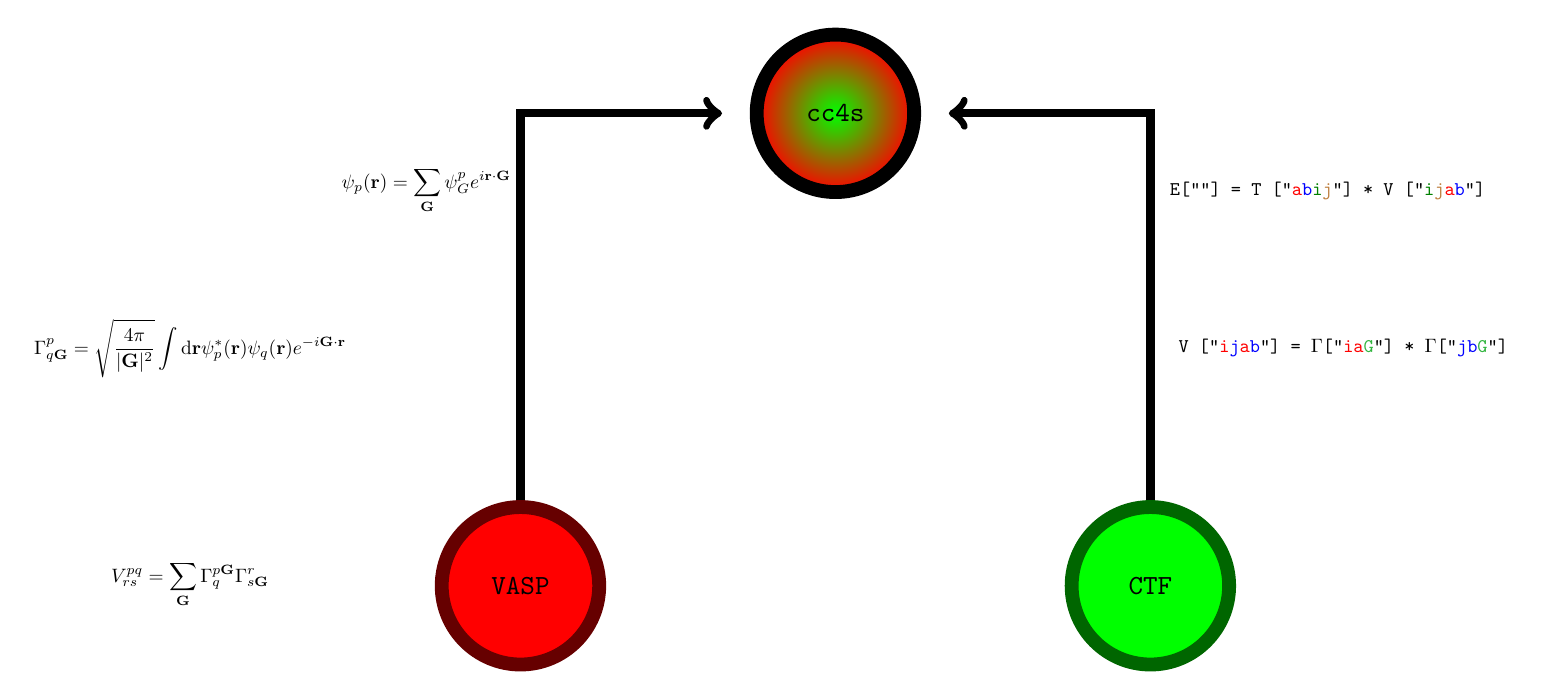
\begin{tikzpicture}[style={
  blob/.style={
    node distance=4cm,
    minimum size=2cm,
  },
  cc4sstyle/.style={
    blob, circle,
    line width=5,
    inner color=green,
    outer color=red,
    draw,
  },
  ctfstyle/.style={
    blob, circle,
    line width=5,
    fill=green,
    draw=green!40!black,
  },
  vaspstyle/.style={
    blob, circle,
    line width=5,
    fill=red,
    draw=red!40!black,
  },
  myarrow/.style={->, shorten >=10pt, line width=3pt}
}]
\draw[]
  node[cc4sstyle] (cc4s) {\texttt{cc4s}}
  node[vaspstyle, below of=cc4s, left of=cc4s, yshift=-2cm] (vasp) {
    \texttt{VASP}
  }
  node[ctfstyle, below of=cc4s, right of=cc4s, yshift=-2cm] (ctf) {
    \texttt{CTF}
  }
;
\def\vaspscale{0.7}
\draw[myarrow]
  (vasp.north) |- (cc4s.west)
  node[pos=0.4, left, scale=\vaspscale] (planewaves) {
    $\displaystyle
    \psi_{p}(\mathbf{r}) =
    \sum_{\mathbf{G}}
      \psi_{G}^{p}
      e^{i \mathbf{r} \cdot \mathbf{G}}
    $
  }
  node[below of=planewaves, xshift=-3cm, node distance=2cm, scale=\vaspscale]
  (gamma) {
    $\displaystyle
    \Gamma^{p}_{q\mathbf{G}} =
    \sqrt{
      \frac{4\pi}{|\mathbf{G}|^{2}}
    }
    \int\mathrm{d}\mathbf{r}
      \psi_{p}^{*}(\mathbf{r})
      \psi_{q}(\mathbf{r})
      e^{-i\mathbf{G} \cdot \mathbf{r}}
    $
  }
  node[below of=gamma, node distance=3cm, scale=\vaspscale]
  (vpqrs) {
    $\displaystyle
    V^{pq}_{rs}
    =
    \sum_{\mathbf{G}}
      \Gamma^{p\mathbf{G}}_{q}
      \Gamma^{r}_{s\mathbf{G}}
    $
  }
;
\def\ctfscale{\vaspscale}
\draw[myarrow]
  (ctf.north) |- (cc4s.east)
  node[pos=0.4, scale=\ctfscale, right] (ctftv) {
    \texttt{
      E[""] =
      T
      ["{\color{red}a}{\color{blue}b}{\color{green!50!black}i}{\color{brown}j}"] *
      V
      ["{\color{green!50!black}i}{\color{brown}j}{\color{red}a}{\color{blue}b}"]
    }
  }
  node[below of=ctftv, xshift=0.2cm, node distance=2cm, scale=\ctfscale] {
    \texttt{
      V
      ["{\color{red}i}{\color{blue}j}{\color{red}a}{\color{blue}b}"]
      =
      $\Gamma$["{\color{red}ia}{\color{yellow!20!green}G}"]
      *
      $\Gamma$["{\color{blue}jb}{\color{yellow!20!green}G}"]
    }
  }
;
\end{tikzpicture}
\end{document}
